%\section{Architecture du projet}    
\chapter{Architecture du projet}
\markboth{\MakeUppercase{Architecture du projet}}{}

	\section{Schéma UML}

		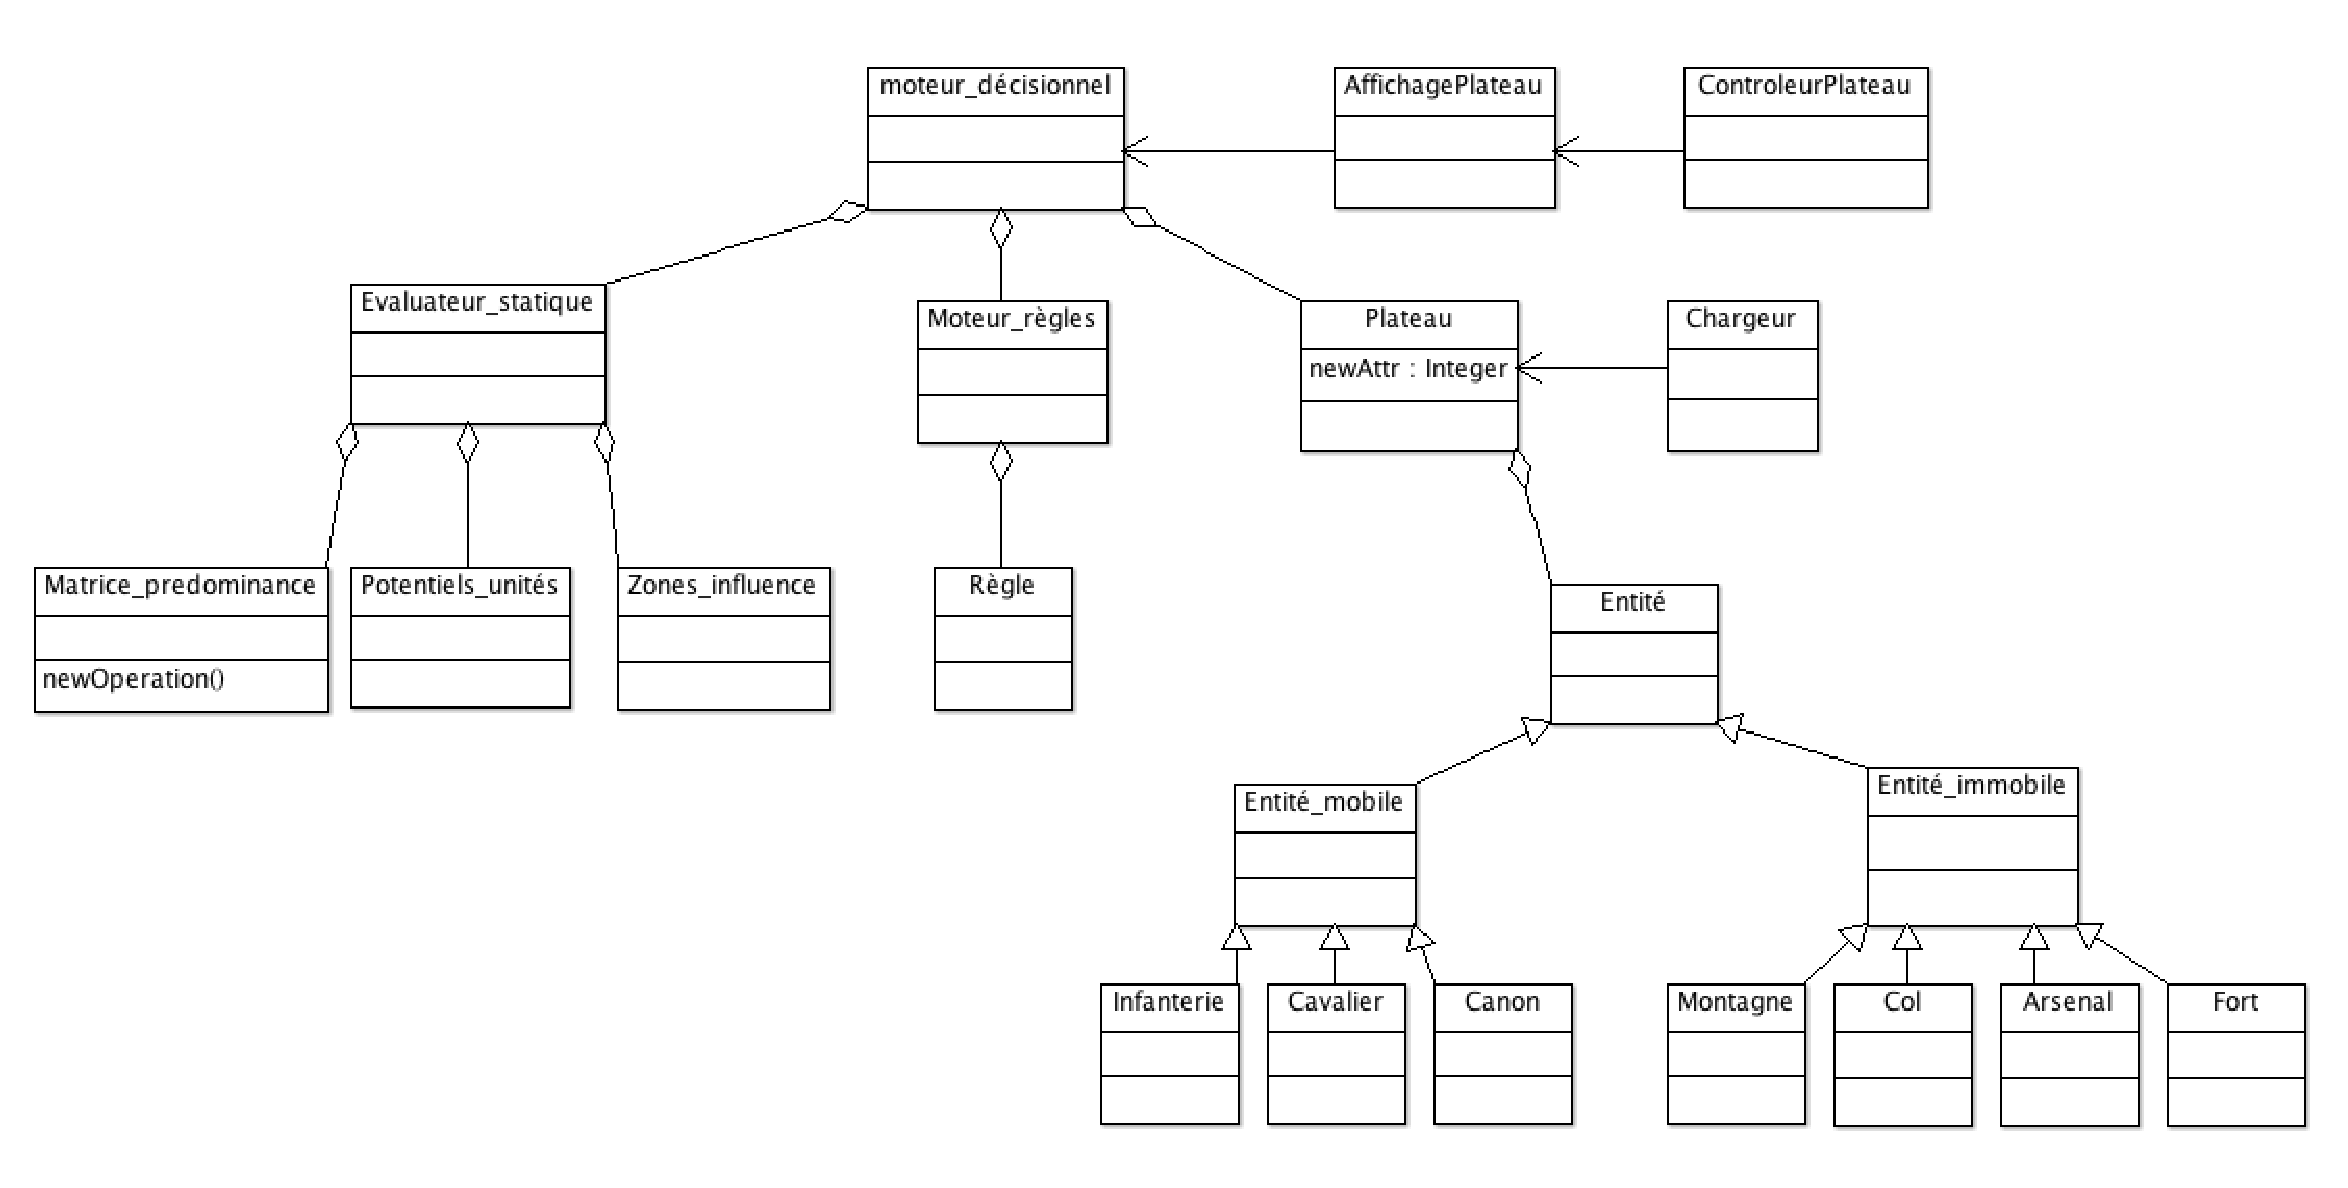
\includegraphics[scale=0.4]{images/diag_classes.eps}

		\clearpage

	\section{Description des classes}

		\subsection*{Board}
		
			\paragraph{Définition :}
			Le Board est une matrice de taille fixe représentant une situation de jeu.
			\paragraph{Interaction :}
			Certaines cases du Board contiendront des objets de type Entity.
			

		\subsection*{EntityLoader}

			\paragraph{Définition :}
			Classe permettant de charger une partie à partir d'un fichier.
			Elle permet de parcourir un fichier ligne par ligne pour parser les informations et les insérer dans le Board.
			\paragraph{Interaction :}
			L'EntityLoader interagit avec le Board en placant directement les objets dans la matrice du Board.

		\subsection*{Entity}

			\paragraph{Définition :}
			Les Entity représentent les éléments de jeu (les unités ainsi que les batiments et obstacles).
			\paragraph{Interaction :}
			Toutes les Entity seront disposées à l'intérieur d'une matrice dans la classe Board.

		\subsection*{MovableEntity}

			\paragraph{Définition :}
			Les MovableEntity sont les unités movibles telles que les infanteries, les cavaliers, les canons ou toute autre unité 
			qu'il est possible de déplacer.
			\paragraph{Interaction :}
			Les MovableEntity seront disposées à l'intérieur d'une matrice dans la classe Plateau.

		\subsection*{UnmovableEntity}

			\paragraph{Définition :}
			Les UnmovableEntity sont des entités présentes sur le plateau mais que les règles ne permettent pas de déplacer. 
			Les forts, les arsenaux, les montagnes ou les cols sont par exemple des UnmovableEntity.
			\paragraph{Interaction :}
			Les UnmovableEntity seront disposées à l'intérieur d'une matrice dans la classe Board. 
			Certaines UnmovableEntity pourront par ailleurs contenir des MovableEntity. (exemple : les forts)

		\subsection*{Engine}

			!!!!!!!!!!!! A COMPLETER !!!!!!!!!!!!
			\paragraph{Définition :}
			Cette classe représente le moteur de règles et fait l'intermediaire entre les faits (la situation de jeu actuelle) 
			et les règles qui sont implémentées dans un fichier ".drl".
			\paragraph{Interaction :}
			L'Engine interagit avec les entités du Board pour modifier certains attributs.

		\subsection*{Rule}

			!!!!!!!!!!!! A COMPLETER !!!!!!!!!!!!
			\paragraph{Définition :}
			Une règle sera une expression logique associée à un fait. Elles ne seront en fait pas codées sous forme de classe mais 
			sous forme de fichier en ".drl".
			\paragraph{Interaction :}
			Les règles seront envoyées à l'Engine qui devra se charger de les appliquer.

		\subsection*{InfluenceArea}

			\paragraph{Définition :}
			Cette classe permettra de calculer les zones d'influence des unités, c'est à dire l'ensemble des cases sur lesquelles 
			chaque unité peut agir.
			\paragraph{Interaction :}
			La classe InfluenceArea aura besoin d'un objet de type Board pour faire ses calculs et stockera les résultats dans 
			les entités elles-mêmes.

		\subsection*{Potential}

			\paragraph{Définition :}
			Cette classe permettra de calculer les potentiels offensifs et défensifs des unités en fonction de leur configuration spatiale.
			\paragraph{Interaction :}
			La classe Potential aura besoin d'un objet de type Board pour faire ses calculs et stockera les résultats dans les 
			entités elles-mêmes.

		\subsection*{DangerousnessMatrix}

			!!!!!!!!!!!! A COMPLETER - Ne va même pas exister ? !!!!!!!!!!!!
			\paragraph{Définition :}
			Cette classe permettra de stocker la matrice de dangerosité représentant les endroit avantageux ou à éviter.
			\paragraph{Interaction :}
			La classe DangerousnessMatrix ...

		\subsection*{StaticEvaluator}

			!!!!!!!!!!!! A COMPLETER - Ne va même pas exister ? !!!!!!!!!!!!
			\paragraph{Définition :}
			AREFAIRE : Le StaticEvaluator est la classe permettant de calculer et stocker l'ensemble des résultats de nos algorithme 
			d'évaluation statique du jeu.
			\paragraph{Interaction :}
			AREFAIRE : Le StaticEvaluator agit directement sur InfluenceArea, Potential et DangerousnessMatrix puisqu'il se charge 
			de les mettre à jour. Le moteur décisionnel aura quant à lui accès à l'évaluateur pour pouvoir prendre des décisions en fonction 
			des résultats trouvés par l'évaluateur.

		\subsection*{DecisionnalEngine}

			\paragraph{Définition :}
			Le DecisionnalEngine se charge de choisir le coup à jouer en fonction d'une situation de jeu donnée et des résultats 
			du StaticEvaluator.
			\paragraph{Interaction :}
			Le DecisionnalEngine interagira avec le Board pour connaître la situation de jeu et les Entity pour connaître les 
			différentes données calculées par le StaticEvaluator.

		\subsection*{BoardDisplayer}

			\paragraph{Définition :}
			Ceci est la classe principale de l'interface graphique. Elle se charge d'afficher les données (Entités et valeurs calculées)
			et contient le MenuDisplayer.
			\paragraph{Interaction :}
			Le BoardDisplayer récupère les données contenues dans le Board afin de pouvoir les afficher, il récupère également des données qui sont calculées
			par le moteur de règles pour chaque entité et stockées dans les entités.

		\subsection*{MenuDisplayer}

			\paragraph{Définition :}
			C'est la deuxième classe formant l'interface graphique. Elle contient les boutons et checkboxes qui permettent
			de régler les paramètres d'affichage. Elle permet également de déclencher le chargement d'un fichier.
			\paragraph{Interaction :}
			Le MenuDisplayer modifie les paramètres d'affichage contenus dans le BoardDisplayer lorsque l'utilisateur clique
			sur les éléments du menu ou utilise des raccourcis clavier.

	\section{Librairie Drools}

		\subsection{Présentation}
			Drools est un moteur de règles, c'est à dire que c'est un système dans lequel il y a des règles qui sont appliquées à des données. 
			Les règles et les données sont ajoutées	à un moteur d'inférence afin qu'il puisse déterminer les règles applicables aux données et ainsi aboutir à une conclusion qui résulte en une action.
			Le moteur de règles s'occupe de bien agencer les règles afin d'optimiser l'exécution (Agenda).

		
			\begin{figure}[!h]
			    \caption{Schéma du fonctionnement de Drools}
			    \centering
			    \includegraphics[width=\textwidth]{images/architecture/drools_schema.ps}
			\end{figure}
	

		\subsection{Les avantages}
			L'utilisation d'un moteur de règles nous permet de pouvoir séparer la logique et les données de sorte à ce que le maintien de l'application soit plus facile dans le futur.
			\\
			Avec cette librairie nous pouvons centraliser la gestion des connaissances dans des fichiers de règles dont l'extension est {\itshape drl}.
			\\
			Cette librairie utilise l'algorithme de Rete afin de trouver les règles en fonction des données. Cela assure un maintien de la rapidité même si nous avons de nombreuses règles.
			\\
			Drools nous permet de nous concentrer sur le « Qu'est ce que je dois faire » plutot que sur le « Comment le faire ».


		\subsection{Exemple d'utilisation}

